

\documentclass[runningheads,a4paper,10pt]{etc/llncs}
\usepackage{amssymb}
\usepackage{graphicx}
\usepackage{hyperref}

\usepackage{url}
\usepackage{float}
\usepackage{chngpage}
\usepackage{listings}
\usepackage{apacite}

\usepackage[utf8]{inputenc}
% \usepackage[spanish,activeacute]{babel}

\usepackage{longtable}
\usepackage{makecell}


\let\stdsection\section
\renewcommand\section{\newpage\stdsection}
\usepackage[backend=biber,style=alphabetic,sorting=ynt]{biblatex}
\addbibresource{citations.bib}

\urldef{\mailsa}\path|federico.scenna@gmail.com|    
\newcommand{\keywords}[1]{\par\addvspace\baselineskip
\noindent\keywordname\enspace\ignorespaces#1}

\authorrunning{Lic. Federico Scenna}% Part of LEFT running header
\titlerunning{Análisis de grafos del mercado de criptomonedas}% Part of RIGHT running header

\mainmatter  % start of an individual contribution

% first the title is needed
\title{Análisis de grafos del mercado de criptomonedas}

\author{Lic. Federico Scenna\\ [1cm] {\small Tutor: Dr. Ricardo Maronna}}


\institute{ Maestría en Exploración de Datos y Descubrimiento del Conocimiento \\
Facultad de Ciencias Exactas y Naturales\\ Universidad de Buenos Aires\\
\mailsa
}
\setcounter{tocdepth}{3}


\begin{document}
\let\oldaddcontentsline\addcontentsline
\def\addcontentsline#1#2#3{}
\maketitle
\def\addcontentsline#1#2#3{\oldaddcontentsline{#1}{#2}{#3}}

\newpage

\paragraph{Resumen} En este trabajo se analizan series diarias de precios de distintas criptomonedas entre Agosto del año 2020 y Abril de 2021. A partir de correlaciones
de retornos diarios se visualizaron las relaciones entre los distintos activos. Se
identificaron mayoritariamente altas correlaciones entre los movimientos de pre-
cios y, durante el periodo analizado, el activo Cardano (ADA) como el activo de
referencia del mercado.

\paragraph{Palabras clave} Análisis de grafos, mercados financieros, criptomonedas, blockchain

\tableofcontents

\newpage
\section{Introducción}

Si bien existen aplicaciones de grafos para analizar activos financieros tradicionales tanto para mercados singulares \cite{grekmarket} como dinámicas en los mercados internacionales \cite{towards}. Si bien existen algunos estudios que analizan las propias blockchains \cite{btc-btccash} no hay casos tan extendidos para el caso de los criptoactivos (ver \cite{cryptocurrency_rjc} y \cite{cryptonetwork}). 

\section{Metodología}

\subsection{Fuentes de información}
El objetivo de este trabajo fue analizar los 50 criptoactivos de mayor vo-
lumen de mercado del periodo entre 22 de Agosto 2020 y el 24 de Abril 2021. Se descargaron
series de precios del sitio coinmarketcap.com a través de la libreria de R crypto \footnote{Disponible en: $https://www.rdocumentation.org/packages/crypto/versions/1.1.3$}.


De esta manera, se obtuvo una lista de activos tanto volátiles como estables (estos últimos fueron diseñados para mantener un valor similar al dólar estadounidense). Se estableció a que tipo de activo pertenecía cada uno para identificarlo en el grafo.
Tanto los datos como el código de este trabajo se encuentran disponibles un repositorio de Github\footnote{$https://github.com/FedeScenna/Crypto_NetworkAnalysis$}.

\begin{figure}[htp]
    \centering
    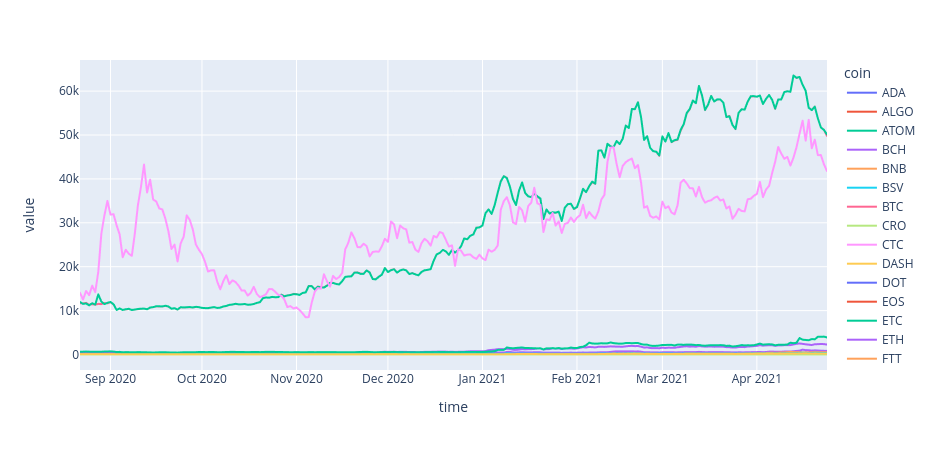
\includegraphics[scale=0.3]{images/volatilecoins_lineplot.png}
    \caption{Precios de monedas volátiles}
    \label{fig:stablecoins}
\end{figure}

\begin{figure}[htp]
    \centering
    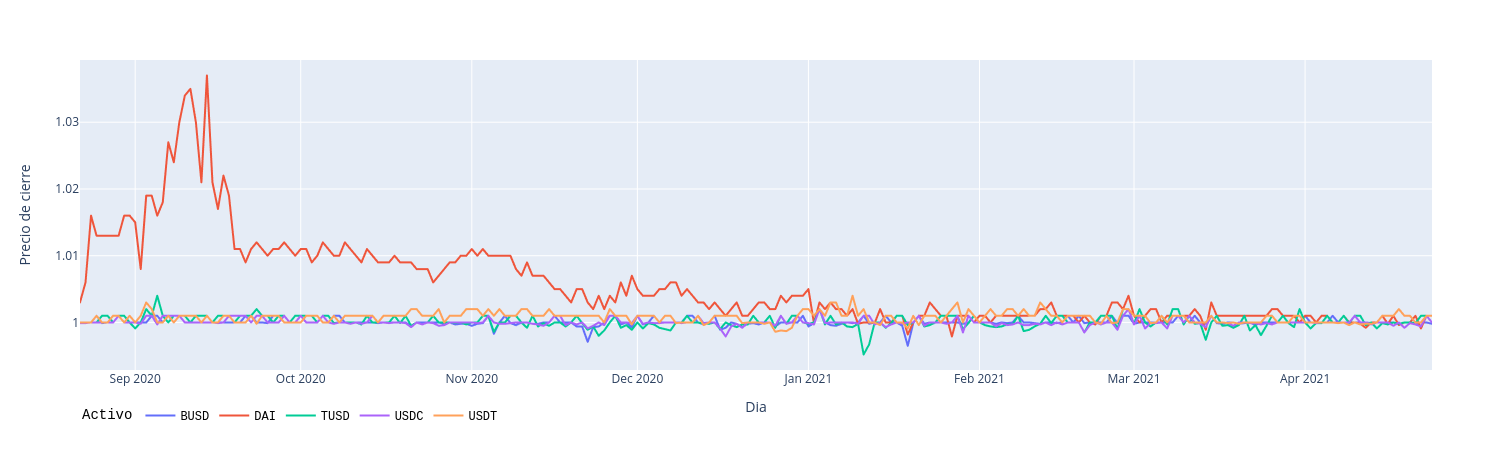
\includegraphics[scale=0.3]{images/stablecoins_lineplot.png}
    \caption{Precios de monedas estables}
    \label{fig:stablecoins}
\end{figure}


\subsection{Transformacion de datos}
Previamente a la construcción del grafo, era necesario establecer alguna
métrica para desestacionalizar la serie de precios de los activos para evitar correlaciones espurias. Uno de los métodos más frecuentes que propone la literatura \cite{cryptonetwork} es la tasa de retorno logarı́tmica:

\begin{math}
log(p_t) -log(p_t-1)
\end{math}

Se decidió, a modo de mantener la claridad en el análisis y por las cualidades
propias del este tipo de mercado, computar retornos diarios de cada uno de los
activos.

A partir de esta métrica de retorno, se calculó la matriz a partir de la correlación de Pearson: 

\begin{figure}[htp]
    \centering
    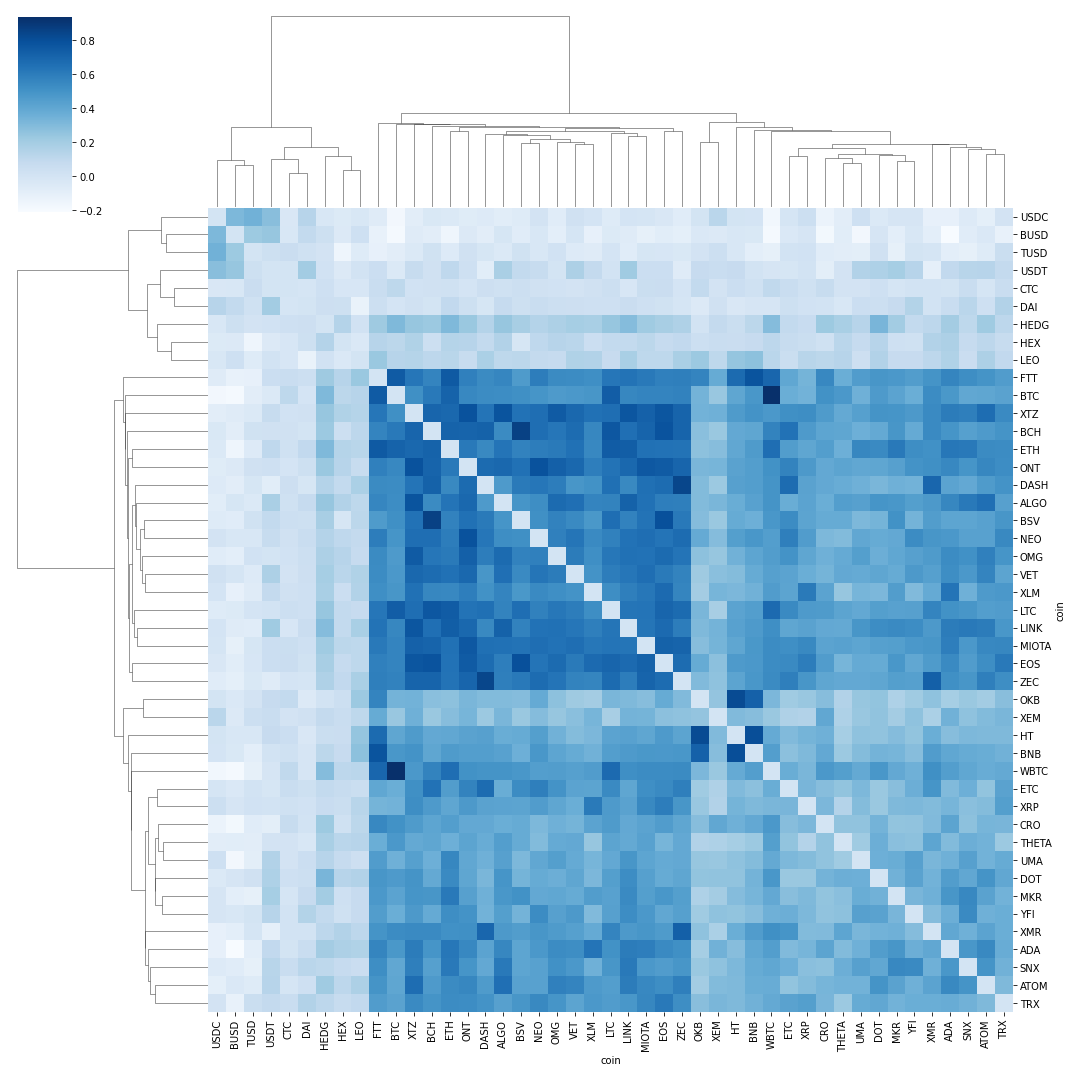
\includegraphics[scale=0.3]{images/corr_matrix.png}
    \caption{Matriz de correlación de los activos}
    \label{fig:corr_matrix}
\end{figure}


\subsection{Construcción de grafos} 

Analizando la distribución de las correlaciones entre todos los activos da a entender que las correlaciones siguen una forma bimodal.

\begin{figure}[htp]
    \centering
    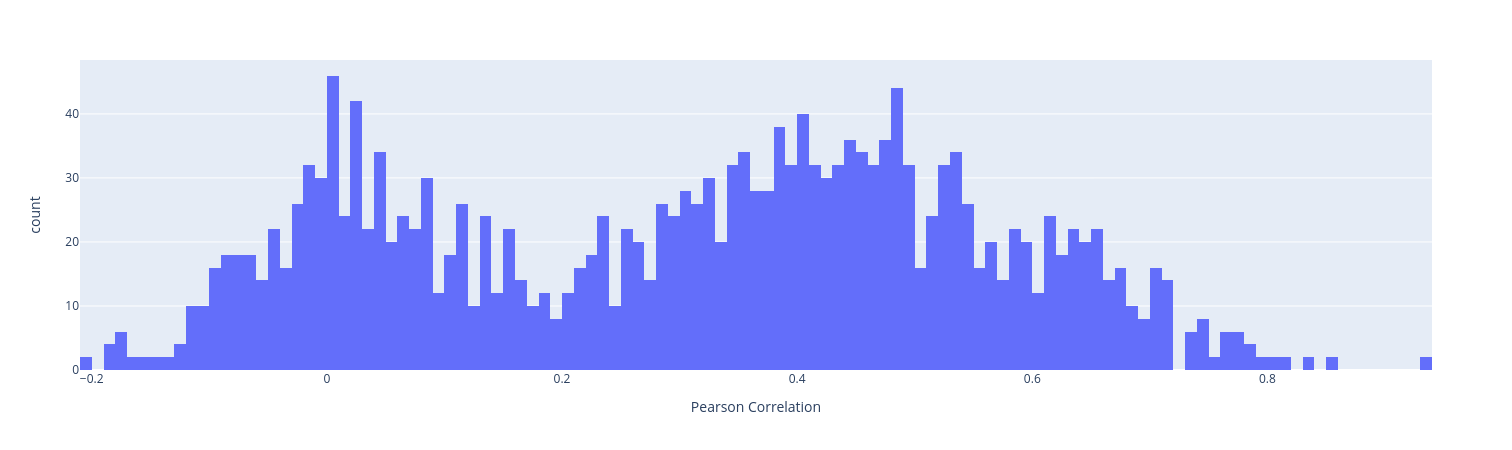
\includegraphics[scale=0.3]{images/correlation_hist.png}
    \caption{Histograma de correlación de los activos}
    \label{fig:hist_corr}
\end{figure}

En la literatura, la metodologı́a usualmente propuesta es la creación de un grafo a partir de una matriz de correlación con un punto de corte determinado.
En base a la distrubición de la correlación y a la centralidad de intermediación (betweenness centrality) promedio de la red, se tomo como valor de corte las aristas entre activos con una correlación mayor al 20\%.

\begin{figure}[htp]
    \centering
    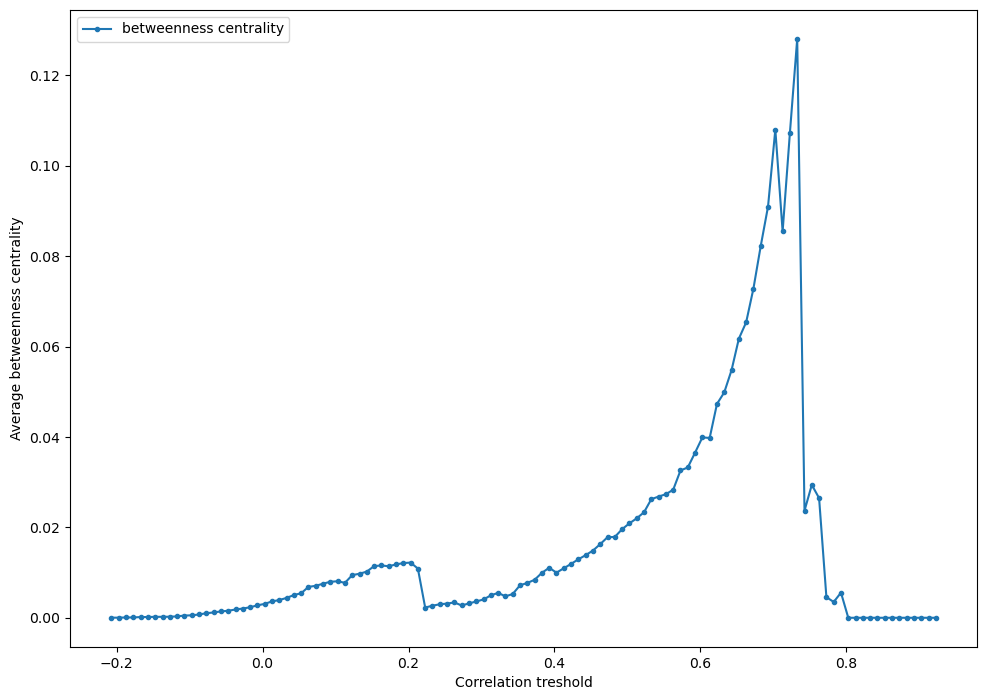
\includegraphics[scale=0.3]{images/betweeness_centrality.png}
    \caption{Ćentralidad de intermediación}
    \label{fig:btw_centrality}
\end{figure}


A partir de este punto de corte y consistente con la literatura, se construyó un Minimum Spanning Tree (MST) que puede visualizarse a continuación:

\begin{figure}[htp]
    \centering
    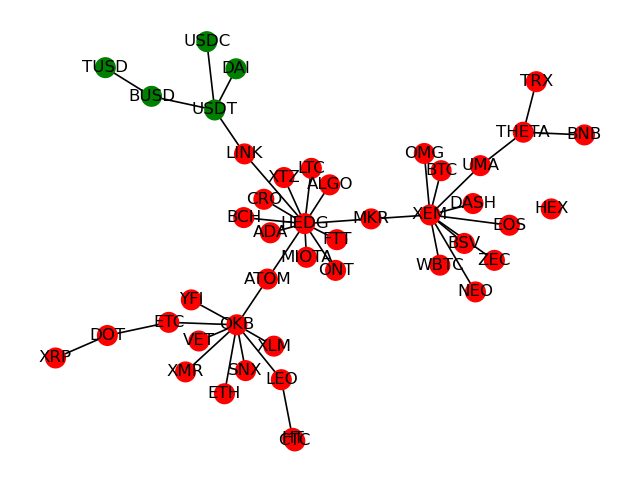
\includegraphics[scale=1]{images/mst.png}
    \caption{MST de los activos}
    \label{fig:hist_corr}
\end{figure}

A partir de esta estructura, se puede visualizar las distancias relativas de los nodos en función de la correlación que tienen entre si. De tal manera, cuan más cerca se encuentren dos nodos mayor es la correlación que existe entre ellos. 

\subsection{Búsqueda de comunidades}

Se realizó una búsqueda de comunidades. Se utilizó el algoritmo Louvain cuya modularidad de 0.68 arrojó mejores resultados que Girvan-Neuman. En la imagen siguiente se puede visualizar el resultado de las comunidades encontradas por este algoritmo. El mismo pudo separar adecuadamente los activos estables de los volátiles.


\begin{figure}[htp]
    \centering
    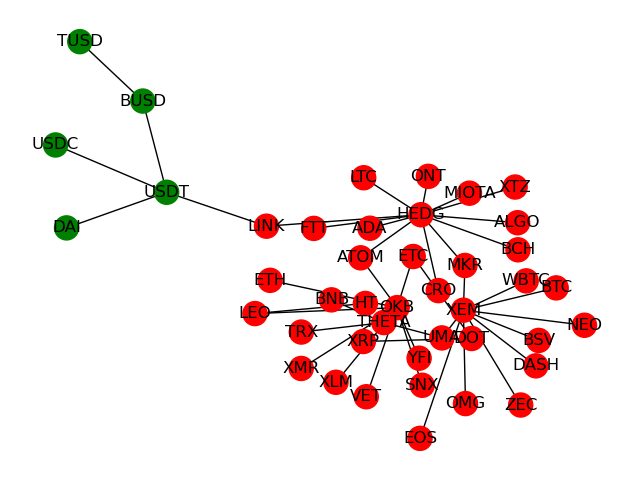
\includegraphics[scale=1]{images/community_louvain.png}
    \caption{Resultado del algoritmo Louvain}
    \label{fig:hist_corr}
\end{figure}

\section{Resultados}

En el caso puntual de este trabajo, hay algunas cualidades que deben resaltarse. En primer lugar, se diferencia claramente entre las monedas estables (resaltadas en verde) y las monedas volátiles (en rojo). 

En segundo lugar, observamos que hay dos activos que se encuentran visiblemente desacoplados del resto de los activos del grafo: CTC (Creditcoin) y HEX (Hex.com). El primero es un token de una blockchain destinada a facilitar capital de crédito y trazabilidad de transacciones a fintechs y a proyectos de microfinanzas. El segundo es un proyecto de finanzas descentralizadas destinado a ofrecer alto interés por depósitos a plazo fijo. Sin embargo, han surgido algunas opiniones cuestionando que pueda afianzarse como un proyecto a largo plazo.

En tercer lugar, se puede observar 4 subgrafos de activos que se encuentran conectados entre sí. Lo que es particularmente interesante son los tres subgrafos de monedas volátiles ya que ni ETH ni BTC son los activos de referencia de esos subgrafos. De esta manera, se constituye una discrepancia respecto a la literatura consultada para este trabajo.

\section{Conclusiones}


\printbibliography[citations]

\end{document}